\chapter{Resultados}
\label{cap:resultados}

Con las decisiones de datos, modelo, umbral y prompt ya cerradas, el capítulo comienza por la selección de los dos métodos de inteligencia artificial y continúa con la comparación de las tres rutas en los dominios sintético y real. También se presentan el coste temporal, el registro WCS y la integración hasta la exportación en formato DXF.

\section{Control de calidad del conjunto sintético}

La puerta de calidad aprobó las 48 hojas del conjunto \texttt{asset\_identity\_v2} sin registrar fallos críticos. El reparto quedó fijado en 24 hojas de entrenamiento, 12 de validación y 12 de prueba. Las 32 identidades de activo fueron únicas y no se encontraron coincidencias entre particiones en sus identificadores, nombres de archivo, hashes de origen, imágenes ni máscaras.

La auditoría también confirmó que todas las rutas existen, que las imágenes conservan las dimensiones de 2100 por 2970 píxeles y que las máscaras binarias y de instancia son válidas. Cada partición contiene las cuatro familias semánticas, las seis condiciones de captura y las dos distribuciones previstas.

Las doce hojas de validación reúnen siempre las mismas ocho identidades de ese subconjunto bajo dos distribuciones y seis condiciones. La prueba aplica el mismo esquema a otras ocho identidades. Este diseño permite comparar de forma controlada la respuesta ante las dos distribuciones y las seis condiciones, aunque las doce hojas no representan grupos independientes de productos.

\section{Optimización de Random Forest}

\subsection{Búsqueda y selección}

En la validación cruzada agrupada, C03 obtuvo el mayor Jaccard medio sobre píxeles, con $0{,}9737$. C07 quedó segundo con $0{,}9723$. El orden entre ambos cambió al reconstruir las hojas completas. C07, con umbral 0,55, alcanzó el mejor IoU de validación y mantuvo ocho componentes en todas las láminas.

\begin{table}[htbp]
\centering
\small
\caption{Segunda etapa de selección de Random Forest sobre doce hojas de validación.}
\label{tab:seleccion_rf}
\begin{tabularx}{\textwidth}{p{2.7cm}ccccY}
\toprule
\textbf{Candidato} & \textbf{Umbral} & \textbf{IoU} & \textbf{Dice} & \textbf{Error comp.} & \textbf{Procedencia} \\
\midrule
C07 & 0,55 & \textbf{0,9918} & \textbf{0,9959} & 0,00 & Segundo en validación cruzada \\
Control C00 & 0,60 & 0,9914 & 0,9956 & 0,00 & Configuración de referencia \\
C03 & 0,55 & 0,9913 & 0,9956 & 0,00 & Primero en validación cruzada \\
\bottomrule
\end{tabularx}
\end{table}

La Tabla~\ref{tab:seleccion_rf} muestra por qué la evaluación necesitó dos etapas: una diferencia pequeña sobre píxeles muestreados no basta para anticipar el comportamiento de una hoja completa. El modelo finalmente bloqueado usa 240 árboles, profundidad máxima 20, dos muestras mínimas para dividir, un mínimo de dos muestras por hoja terminal, 50 por ciento de las variables en cada división y ponderación balanceada, con un umbral de 0,55. La Figura~\ref{fig:rf_validacion_completa} recoge el resultado por lámina de los tres finalistas.

\begin{figure}[htbp]
\centering
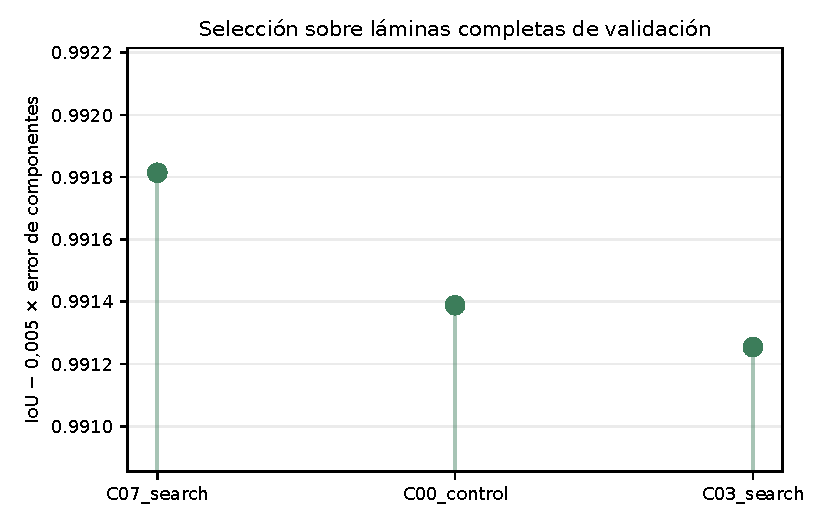
\includegraphics[width=0.93\textwidth]{../resultados/figuras/rf_idv2_full_sheet_validation.pdf}
\caption{IoU de los candidatos finalistas sobre las doce hojas completas de validación. La línea de selección combina solapamiento y error de componentes.}
\label{fig:rf_validacion_completa}
\end{figure}

\subsection{Ablación de características}

La ablación se realizó como diagnóstico sobre 24\,000 píxeles de validación y no intervino en la elección del modelo. Las nueve variables de color alcanzaron un Jaccard de $0{,}9523$. Añadir gradientes elevó el valor a $0{,}9636$, y el conjunto completo de 19 variables llegó a $0{,}9810$. Incorporar las coordenadas absolutas produjo $0{,}9800$. La Figura~\ref{fig:rf_ablacion} reúne esta comparación.

\begin{figure}[htbp]
\centering
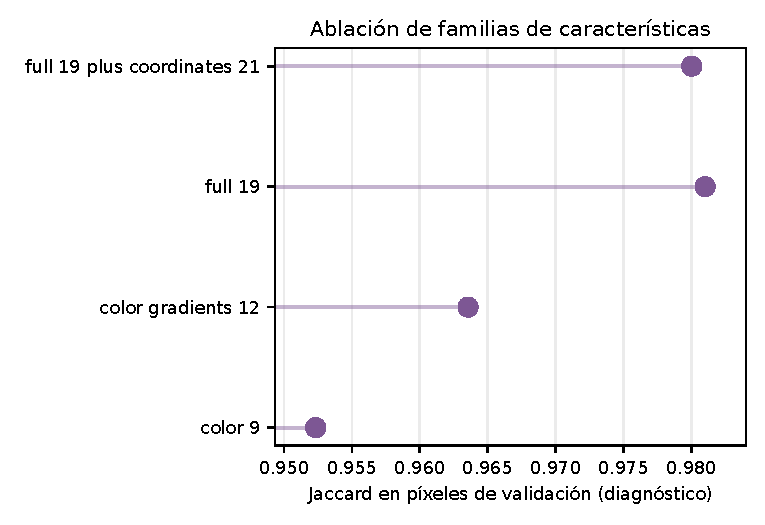
\includegraphics[width=0.86\textwidth]{../resultados/figuras/rf_idv2_feature_ablation.pdf}
\caption{Ablación diagnóstica de las variables de Random Forest sobre validación. El conjunto de 19 variables obtiene el mayor Jaccard en esta corrida, con una diferencia de 0,0010 respecto de la variante que añade coordenadas.}
\label{fig:rf_ablacion}
\end{figure}

La representación de 19 variables ya estaba bloqueada y no se modificó. El diagnóstico fue coherente con no añadir coordenadas: al incorporarlas, el Jaccard pasó de 0,9810 a 0,9800. El ensayo no permite atribuir la diferencia a un tipo concreto de borde, sombra o desenfoque ni establecer un efecto general de las coordenadas.

\section{Selección del margen de SAM 2}

Con cajas obtenidas por el mismo localizador de la aplicación, los cuatro márgenes conservaron ocho componentes. La Tabla~\ref{tab:seleccion_sam} reúne las métricas y la Figura~\ref{fig:sam_margen} representa la media junto con su intervalo de confianza. El 5 por ciento obtuvo el mayor IoU, aunque aventajó al 3 y al 10 por ciento en menos de cuatro diezmilésimas.

\begin{table}[htbp]
\centering
\small
\caption{Selección del margen de caja de SAM 2 sobre doce hojas de validación.}
\label{tab:seleccion_sam}
\begin{tabularx}{0.88\textwidth}{Ycccc}
\toprule
\textbf{Margen} & \textbf{IoU} & \textbf{Dice} & \textbf{Boundary F1} & \textbf{Error comp.} \\
\midrule
5 por ciento & \textbf{0,9232} & \textbf{0,9600} & 0,7663 & 0,00 \\
3 por ciento & 0,9228 & 0,9599 & \textbf{0,7685} & 0,00 \\
10 por ciento & 0,9228 & 0,9599 & 0,7579 & 0,00 \\
0 por ciento & 0,9214 & 0,9591 & 0,7679 & 0,00 \\
\bottomrule
\end{tabularx}
\end{table}

\begin{figure}[htbp]
\centering
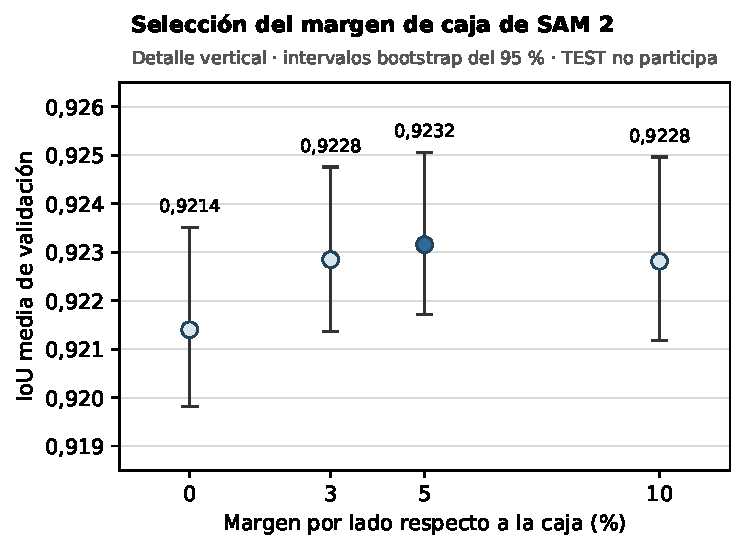
\includegraphics[width=0.82\textwidth]{../resultados/figuras_protocolo_v8/sam2_margin_selection_idv2.pdf}
\caption{Detalle de la IoU media para los cuatro márgenes evaluados. El eje vertical está restringido al intervalo 0,9185--0,9265 para hacer visibles diferencias de hasta 0,0018. Las barras de error son intervalos percentiles \textit{bootstrap} del 95 por ciento y se solapan ampliamente.}
\label{fig:sam_margen}
\end{figure}

El margen del 5 por ciento quedó bloqueado antes de abrir la prueba. Con ese valor, las cajas operativas y las ideales produjeron resultados casi idénticos: IoU de $0{,}92308$ y $0{,}92318$ en prueba, y concordancias de $0{,}95364$ y $0{,}95372$ en real. En las imágenes estudiadas, esta proximidad indica que la localización de las cajas no domina el error final.

\section{Comparación en prueba sintética}

Las doce hojas bloqueadas dejaron una diferencia clara entre el solapamiento de región y la fidelidad del borde. Random Forest encabezó IoU, Dice y Boundary F1, mientras que SAM 2 superó a la línea clásica en las dos métricas de región y la línea clásica conservó mayor coincidencia de contorno. La Tabla~\ref{tab:resultados_sinteticos} reúne los valores y la Figura~\ref{fig:comparacion_idv2} permite ver cómo se distribuyen entre láminas.

\begin{table}[htbp]
\centering
\small
\caption{Resultados finales sobre doce hojas sintéticas con identidades no vistas.}
\label{tab:resultados_sinteticos}
\begin{tabularx}{\textwidth}{Ycccc}
\toprule
\textbf{Método} & \textbf{IoU} & \textbf{Dice} & \textbf{Boundary F1} & \textbf{Error comp.} \\
\midrule
Visión clásica & $0{,}9098 \pm 0{,}0037$ & 0,9528 & 0,8039 & 0,00 \\
Random Forest & $\mathbf{0{,}9879 \pm 0{,}0089}$ & \textbf{0,9939} & \textbf{0,9412} & 0,00 \\
SAM 2 Hiera Tiny & $0{,}9231 \pm 0{,}0072$ & 0,9600 & 0,7376 & 0,00 \\
\bottomrule
\end{tabularx}
\end{table}

\begin{figure}[htbp]
\centering
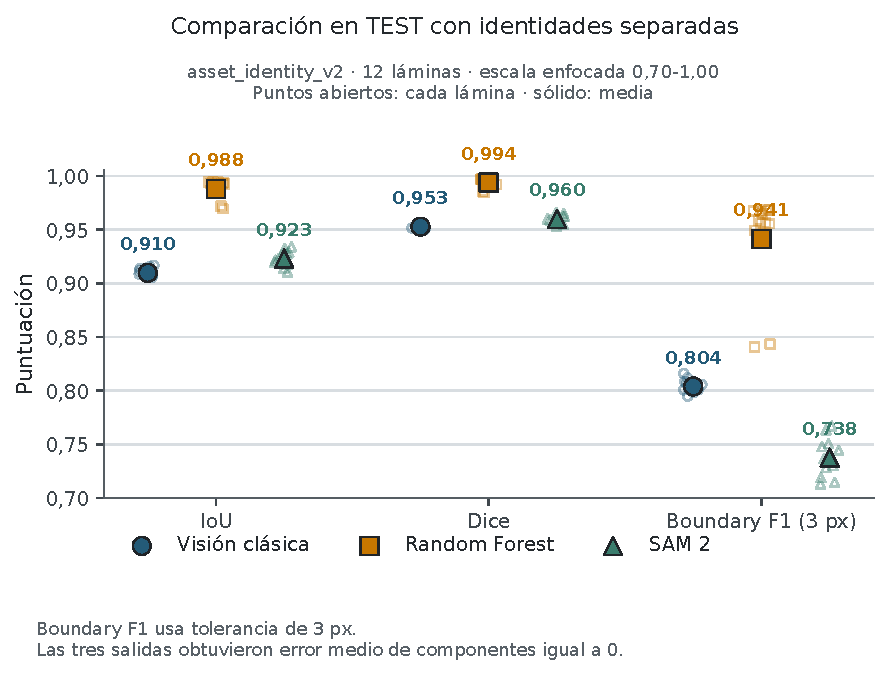
\includegraphics[width=0.96\textwidth]{../resultados/figuras/comparison_test_idv2_final.pdf}
\caption{Comparación de IoU, Dice y F1 de contorno en la prueba sintética con identidades separadas. Los marcadores abiertos corresponden a cada lámina y los sólidos muestran la media.}
\label{fig:comparacion_idv2}
\end{figure}

El desenfoque combinado con ruido de la condición C5 expuso la mayor sensibilidad de Random Forest: su IoU medio descendió a $0{,}9707$, cuando en C1, C2, C3 y C4 superaba $0{,}9917$, frente a $0{,}9839$ bajo la deformación ondulatoria C6. Esa pérdida afectó al solapamiento, pero no al recuento de objetos, pues las doce hojas conservaron el número correcto de componentes.

\section{Concordancia en las capturas reales}

Ningún parámetro se modificó al abrir la evaluación real. Según la Tabla~\ref{tab:resultados_reales}, la visión clásica presentó la mayor concordancia con la referencia canónica asistida. SAM 2 quedó $0{,}0251$ puntos por debajo y mantuvo las ocho instancias en las trece capturas. Random Forest descendió a $0{,}2881$ y produjo una sola región grande en todos los casos.

\begin{table}[htbp]
\centering
\small
\caption{Concordancia con la referencia asistida en trece vistas de una hoja real.}
\label{tab:resultados_reales}
\begin{tabularx}{\textwidth}{Ycccc}
\toprule
\textbf{Método} & \textbf{IoU} & \textbf{Dice} & \textbf{Boundary F1} & \textbf{Error comp.} \\
\midrule
Visión clásica & $\mathbf{0{,}9787 \pm 0{,}0159}$ & \textbf{0,9892} & \textbf{0,9069} & 0,00 \\
Random Forest & $0{,}2881 \pm 0{,}0037$ & 0,4473 & 0,2366 & 7,00 \\
SAM 2 Hiera Tiny & $0{,}9536 \pm 0{,}0083$ & 0,9763 & 0,7200 & 0,00 \\
\bottomrule
\end{tabularx}
\end{table}

Los intervalos percentiles \textit{bootstrap} del 95 por ciento para la media de IoU fueron $[0{,}9696,\,0{,}9863]$ para la línea clásica y $[0{,}9492,\,0{,}9577]$ para SAM 2. Describen la variación observada al remuestrear las trece capturas de una misma hoja y no sustentan una inferencia sobre productos independientes.

La región dominante generada por Random Forest se aprecia en la Figura~\ref{fig:rf_real}. El contraste descriptivo entre los dominios sintético y real se resume en la Figura~\ref{fig:brecha_dominios}, con la cautela de que sus referencias no son equivalentes.

\begin{figure}[htbp]
\centering
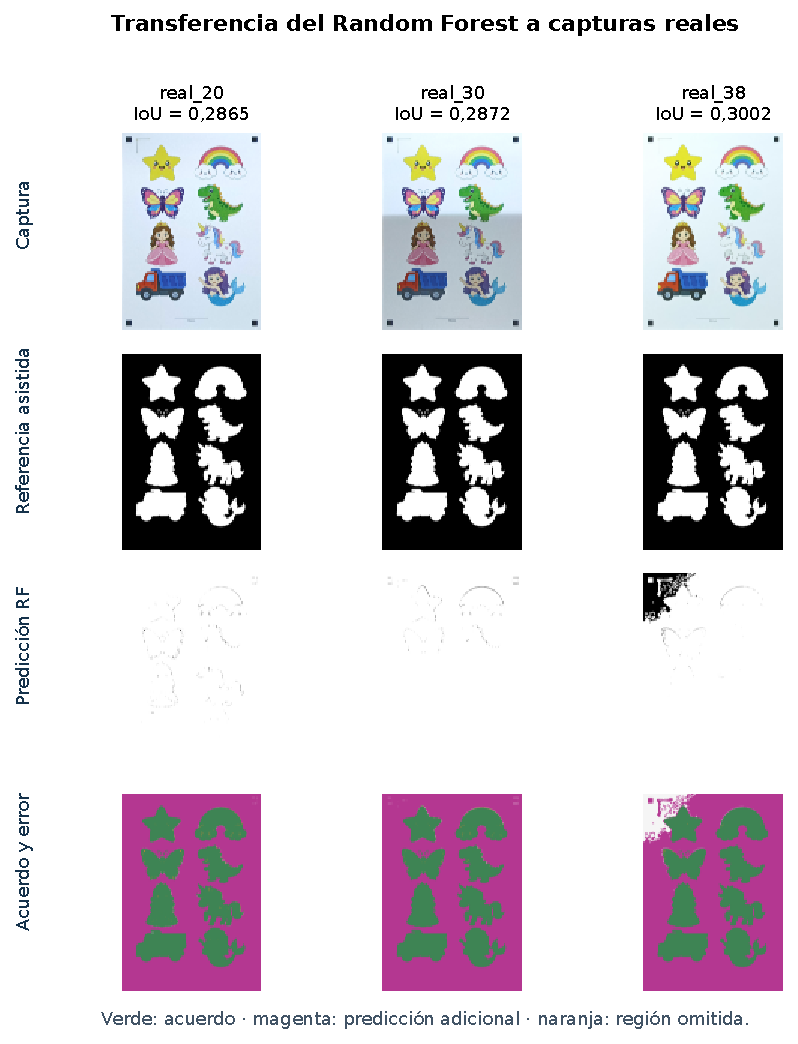
\includegraphics[width=0.94\textwidth]{../resultados/figuras/rf_idv2_real_agreement_examples.pdf}
\caption{Transferencia del Random Forest bloqueado a capturas reales. La predicción se extiende sobre una gran región de papel y no recupera las ocho siluetas.}
\label{fig:rf_real}
\end{figure}

\begin{figure}[htbp]
\centering
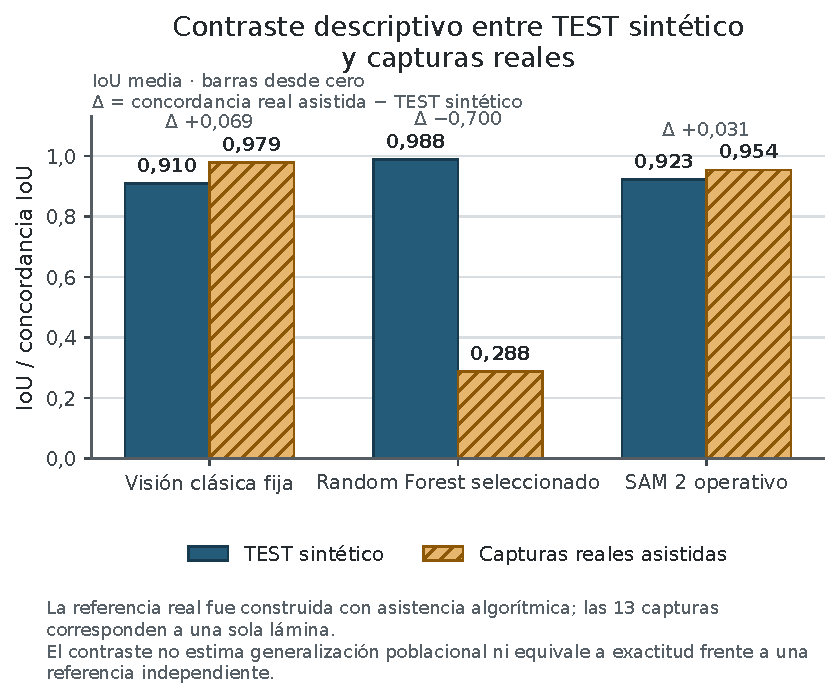
\includegraphics[width=0.94\textwidth]{../resultados/figuras/synthetic_real_gap_final.pdf}
\caption{Contraste descriptivo del IoU en la prueba sintética y de la concordancia IoU en las capturas reales. Las referencias no son equivalentes, por lo que la distancia entre barras documenta el cambio observado, pero no estima por sí sola transferencia ni generalización.}
\label{fig:brecha_dominios}
\end{figure}

\section{Coste temporal}

El banco temporal utilizó cuatro capturas rectificadas y precargadas, con un calentamiento y cinco repeticiones por imagen para cada método. Los tiempos de segmentación, medidos con el alcance homogéneo definido en la metodología, se presentan en la Tabla~\ref{tab:tiempos_segmentacion}.

\begin{table}[htbp]
\centering
\small
\caption{Tiempo de segmentación sobre CPU con imágenes precargadas, veinte mediciones por método.}
\label{tab:tiempos_segmentacion}
\begin{tabularx}{0.88\textwidth}{Yccc}
\toprule
\textbf{Método} & \textbf{Media (s)} & \textbf{Mediana (s)} & \textbf{Desv. (s)} \\
\midrule
Visión clásica & 0,1367 & 0,1330 & 0,0198 \\
Random Forest & 12,7163 & 12,1190 & 1,6652 \\
SAM 2 operativo & 2,1736 & 2,1430 & 0,2161 \\
\bottomrule
\end{tabularx}
\end{table}

Para SAM 2 se cronometró la ruta completa, desde el localizador hasta el postprocesamiento, incluido el codificador de imagen y no solo la decodificación de las cajas. Su media en CPU fue de $2{,}1736$ segundos. Esto equivale a 15,9 veces el tiempo de la línea clásica, mientras Random Forest necesitó 5,9 veces el tiempo de SAM 2. En este último método, los $12{,}7163$ segundos comprenden el cálculo de las 19 variables para más de seis millones de píxeles, la predicción de probabilidades y el postprocesamiento. Como las etapas no se cronometraron por separado, el total no puede atribuirse a una sola de ellas.

\section{Registro WCS y estabilidad entre capturas}

El detector encontró cuatro marcadores en las trece fotografías. Clasificó como válidas las diez que contienen la marca WCS y rechazó las capturas 13, 15 y 17. No hubo falsos positivos ni estados ambiguos en el conjunto real. La Tabla~\ref{tab:wcs_resultados} resume la clasificación y la dispersión observada.

\begin{table}[htbp]
\centering
\small
\caption{Resultado del registro geométrico sobre las capturas reales.}
\label{tab:wcs_resultados}
\begin{tabularx}{0.88\textwidth}{Yc}
\toprule
\textbf{Indicador} & \textbf{Resultado} \\
\midrule
Marcadores detectados & 13 de 13 capturas \\
Clasificación WCS & 10 positivas y 3 negativas, todas correctas \\
Desviación radial media del origen & 0,195 mm \\
Desviación radial máxima del origen & 0,390 mm \\
Desv. estándar del ángulo X & 0,085 grados \\
\bottomrule
\end{tabularx}
\end{table}

\begin{figure}[htbp]
\centering
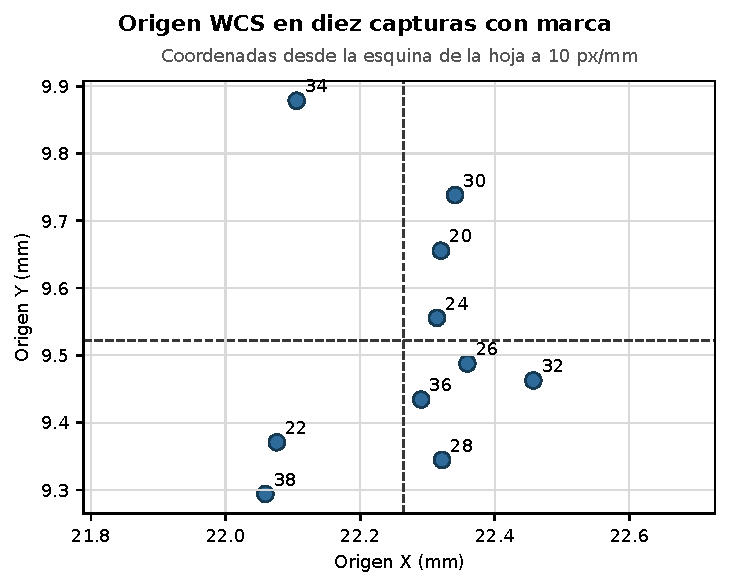
\includegraphics[width=0.80\textwidth]{../resultados/figuras_protocolo_v8/wcs_origin_repeatability_v8.pdf}
\caption{Dispersión del origen WCS recuperado en diez adquisiciones de la misma hoja. El centro representa la media observada, no una referencia metrológica independiente.}
\label{fig:wcs_repetibilidad}
\end{figure}

La Figura~\ref{fig:wcs_repetibilidad} representa la posición del origen recuperado en las diez capturas positivas respecto de su propia media. La estabilidad de máscaras se calculó entre los 45 pares posibles de esas capturas. La línea clásica obtuvo un IoU medio entre pares de $0{,}9644$ y SAM 2 de $0{,}9631$. Random Forest alcanzó $0{,}9883$, pero ninguna captura mantuvo ocho componentes. Esta última cifra describe una equivocación estable y no un mejor contorno.

\section{Integración y validación estructural del DXF}

Los cuatro marcadores se localizaron en las trece capturas y SAM 2 produjo ocho siluetas exteriores en la ruta operativa. El WCS se reconoció como válido en diez capturas y como ausente en tres, tal como correspondía. La aplicación exportó y reabrió los diez DXF autorizados, mientras que en los tres casos sin WCS bloqueó la salida. Así se evitó crear archivos sin una referencia geométrica aceptada. Cada DXF válido contenía ocho trayectorias de corte y no convirtió los vacíos internos de la máscara en perforaciones. Al reabrirlos se comprobaron las capas, el cierre de las polilíneas, la finitud de las coordenadas, el área no nula y unos límites plausibles. El alcance de estas comprobaciones es estructural: no equivale a una validación metrológica ni a una prueba de corte físico.

Las 23 pruebas automatizadas terminaron sin fallos y cubrieron la configuración, la escala, los estados de exportación, la ausencia y la ambigüedad del WCS, las siluetas exteriores, el modo opcional de huecos, el offset y la lectura de retorno del DXF. Con ello se verificó la continuidad entre módulos, aunque no el error entre una trayectoria calculada y un corte físico.
